\part{Capitulo 4}
\vspace{-0.3cm}
\begin{center}
    \begin{large}
        Metodos Probabilisticos y Estadisticos
    \end{large}
\end{center}

La mayor parte de los procesos hidrologicos son aleatorios, no existen procesos puramente deterministicos. En consecuencia, para poder hacer una caracterizacion se \textbf{debe registrar la ocurrencia de ellos} mediante registros historicos, los cuales son sometidos a un post procesado estadistico.
\\ \\
Los objetivos son los siguientes:

\begin{itemize}
    \item Estimacion de P( ) de que ocurra un determinado evento
    \item Estimacion de eventos que no han ocurrido o no se han observado
    \item Caracterizacion estadistica de series hidrologicas
    \item Correlacion y regrecion para completar y extender series
\end{itemize}

\section{Frecuencia Relativa y Acumulada}

La sumatoria de todas las frecuencias relativas debe ser igual a 1, es decir:

\begin{equation}
    \sum_{i=1}^{n} f_i = 1
\end{equation}

Estas funciones son obtenidas a partir de una muestra, por lo que se pueden obtener de estimaciones de la poblacion aproximando como limites:

\begin{figure}[H]
    \centering
    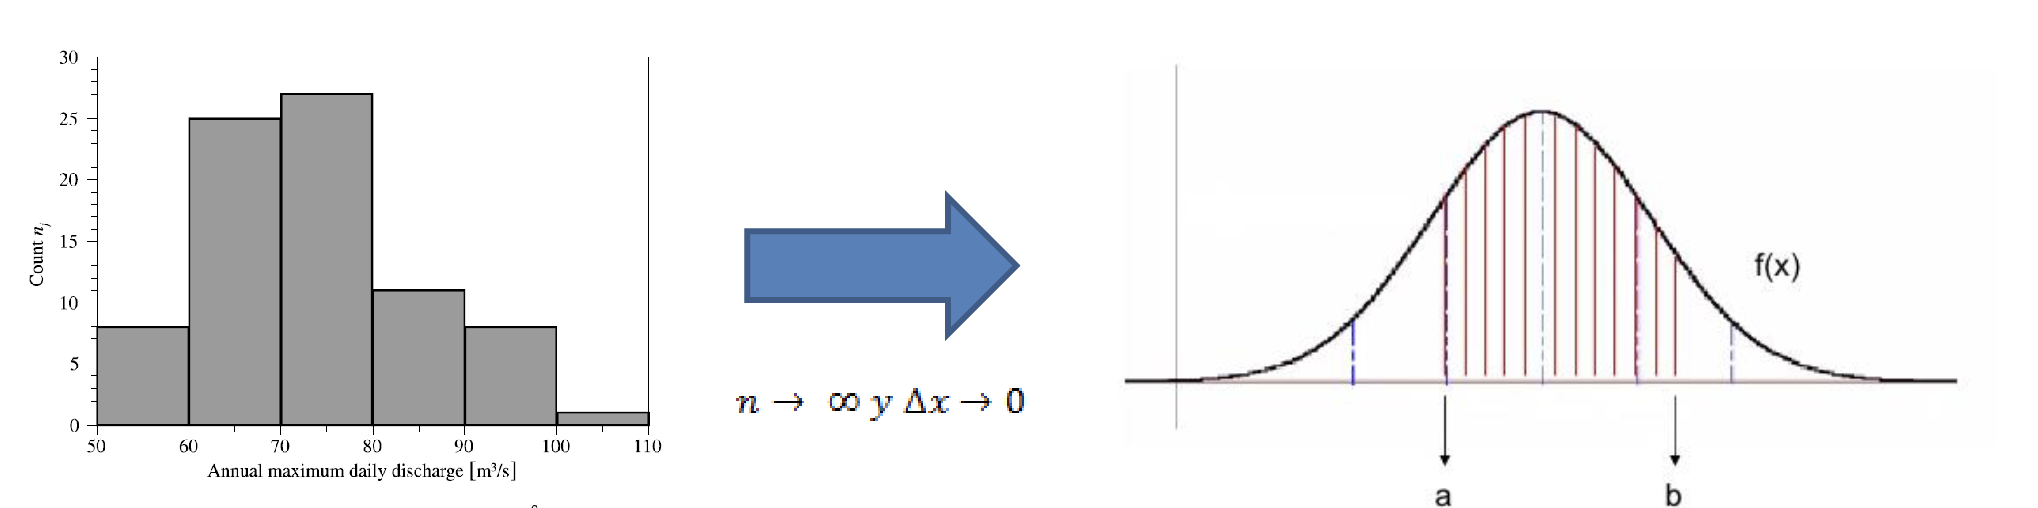
\includegraphics[width=0.85\textwidth]{imagenes/frecuencia.png}
    \label{fig:frecuencia_acumulada}
\end{figure}

\section{Periodo de Retorno y P( ) de Excedencia}

Se puede definir como: el intervalo de recurrencia promedio entre evnetos que igualan o excedan una magnitud especifica
\\ \\
Es decir, en un horizonte de tiempo grande, se esperaria observar eventos iguales o mayores cada \textbf{T años}.
\\ \\
Sea \textbf{p} la probabilidad de exito y \textbf{(1-p)} la probabilidad de falla en un determinado año. Podemos definir la \textbf{probabilidad de recurrencia $\pi$} como el producto de \textbf{$\pi$ - 1} fallas seguidas por un exito, por lo tanto:

\begin{equation}
    P(X > X_t) = \frac{1}{T}
\end{equation}

Ejemplo:

\begin{figure}[H]
    \centering
    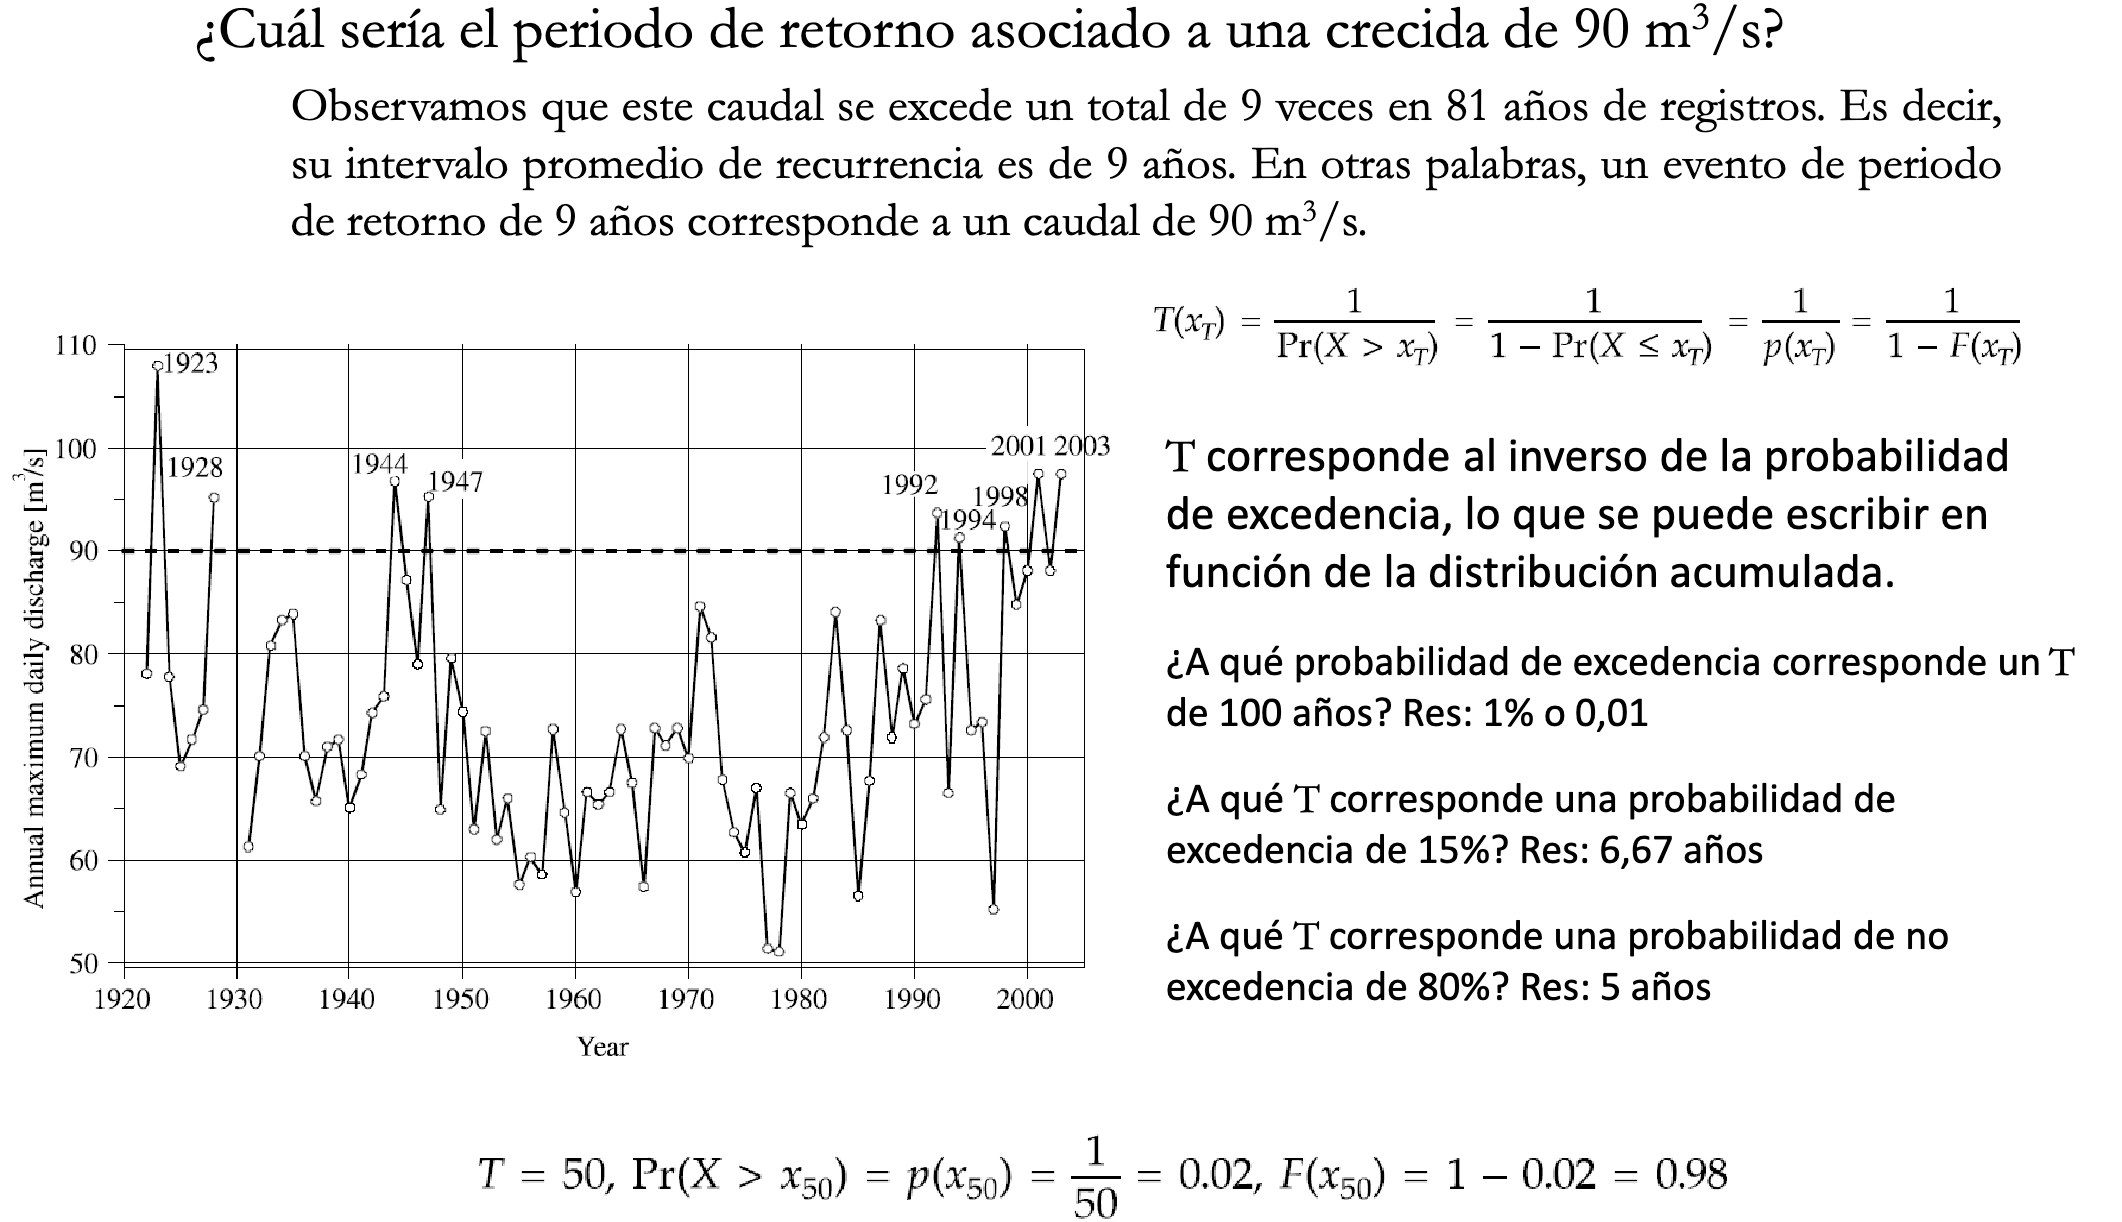
\includegraphics[width=0.85\textwidth]{imagenes/retorno.png}
    \label{fig:periodo_retorno}
\end{figure}

\section{Seguridad y Riesgo Hidrololgico}

Se define como la probabilidad de no excedencia:

\begin{equation}
    P_{no-exc} = 1 - \frac{1}{T}
\end{equation}

Por lo tanto, la probabilidad de que cierto valor no se exceda en n años es:

\begin{equation}
    S = (1 - \frac{1}{T})^n 
\end{equation}

Lo cual se define como \textbf{Seguridad Hidrologica}, donde su complemento es el \textbf{Riesgo Hidrologico}, lo cual se usa para obras hidraulicas:

\begin{equation}
    R = 1- S = 1 - (1 - \frac{1}{T})^n
\end{equation}

\textbf{Nota: aproximar el valor de t a un valor multiplo de 5}

\section{Distribuciones Discretas}

\subsection{Bernoulli}

Una variable aleatoria posee dos estados, exito o fracaso, por lo tanto puede ser 1 o 0. Por lo tanto:

\begin{equation}
    P(X = 1) = p
\end{equation}

\begin{equation}
    P(X = 0) = 1 - p
\end{equation}

\subsection{Distribucion Binomial}

Este modelo surge a partir de la realizacion de n ensayos independientes tipo bernoulli, donde se define una variable aleatorioa k como el numero de exitos que ocurren en n ensayos, por lo tanto:

\begin{equation}
    P(X = k) = \binom{n}{k} \cdot p^k \cdot (1-p)^{n-k}
\end{equation}

Donde:

\begin{equation}
    \binom{n}{k} = \frac{n!}{k!(n-k)!}
\end{equation}

Y K es el numero de evnetos exitosos.
\\ \\
Cada evento climatologico es independiente, por lo tanto es un ensayo tipo bernoulli, y su conjunto se representa binomialmente

\section{Parametros Estadisticos}

\subsection{Varianza}

Se denomina a la varianza \textbf{$s^2$} como la media de los cuadrados de las diferencias entre cada valor y la media, por lo tanto:
\\ \\
Caso discreto: 

\begin{equation}
    s^2 = \frac{\sum_{i=1}^{n} (x_i - \bar{x})^2}{n-1}
\end{equation}

Caso continuo:

\begin{equation}
    \sigma^2 = E((x-\mu)^2)
\end{equation}

\subsection{Desviacion Estandar}

Se define como la raiz cuadrada de la varianza, por lo tanto:

\begin{equation}
    s = \sqrt{s^2}
\end{equation}

\subsection{Coeficiente de Variacion}

Se define como la relacion entre la desviacion estandar y la media, por lo tanto:

\begin{equation}
    CV = \frac{s}{\bar{x}}
\end{equation}

\subsection{Coeficiente de Asimetria}

Se define como la medida de asimetria de una distribucion, por lo tanto:

\begin{equation}
    \gamma = \frac{E((x-\mu)^3)}{\sigma^3}
\end{equation}

\section{Distribuciones Continuas}

\subsection{Distribucion Normal}

Se define como:

\begin{equation}
    f(x) = \frac{1}{\sigma\sqrt{2\pi}} \cdot e^{-\frac{(x-\mu)^2}{2\sigma^2}}
\end{equation}

Donde $\mu$ es la media y $\sigma$ la desviacion estandar.
\\ \\
Esta funcion no es integrable, por lo tanto para evaluar la funcion se utilizan tablas y o formulas aproximadas.
\\ \\
\textbf{El proceso de normalizacion consiste en reemplazar la variable original por una nueva variable estandarizada (z) }

\begin{equation}
    z = \frac{x-\mu}{\sigma}
\end{equation}

De esta forma se obtiene:

\begin{equation}
    f(x) = \frac{1}{\sqrt{2\pi}} \cdot e^{-\frac{z^2}{2}}
\end{equation}

\subsection{Distribucion Log Normal}

Es una transformacion de la distribucion Normal, donde se modela de una forma asimetrica con respecto a un valor medio, por ejemplo para precipitaciones o caudales:

\begin{equation}
    f(x) = \frac{1}{\sigma_y\sqrt{2\pi}} \cdot e^{\frac{1}{2}(\frac{y-\mu_y}{\sigma_y})^2}
\end{equation}

Donde los parametros se estiman en base a la muestra aplicando log a las variables observadas:

\begin{equation}
    \mu_y = \bar{y} = \frac{1}{N} \sum_{i=1}^{N} \ln(x_i)
\end{equation}

\subsection{Distribución de Valores Extremos}

Los datos en hidrología suelen ser series de valores extremos o excedencias anuales (máximos o mínimos).

Distribución de Valor Extremo General (DVEG):

\begin{equation}
    F(x) = \exp \left\{ - \left[ 1 - \kappa \left( \frac{x - u}{\alpha} \right) \right]^{1/\kappa} \right\}
\end{equation}

Existen 3 tipos de distribuciones extremas:

\begin{enumerate}
    \item Gumbel: $\kappa = 0$ en DVEG
    \begin{equation}
        F(x) = \exp\left[-\exp\left(-\frac{x-u}{\alpha}\right)\right]
    \end{equation}
        
    \begin{equation}
        \alpha = \frac{\sqrt{6} \cdot \sigma}{\pi}
        \quad \text{y} \quad
        u = \bar{x} - 0.5722 \cdot \alpha
    \end{equation}

    Variable reducida:

    \begin{equation}
        y = \frac{x-u}{\alpha}
    \end{equation}

    Finalmente:

    \begin{equation}
        y_T = -\ln(-\ln\left(\frac{T-1}{T}\right))
    \end{equation}

    \begin{equation}
        x_T = u + \alpha \cdot Y_T
        \quad \text{;} \quad
        Y_T \rightarrow y = \frac{x-u}{\alpha} 
    \end{equation}

    Esta expresión permite calcular el valor asociado a un evento de periodo de retorno T, en función del promedio, desv. estándar y T.

    \item Fretcher: $\kappa < 0$
    \item Weibull: $\kappa > 0$
\end{enumerate}






